\noindent {\em Auteurs: Laura Vranken }
\\
\\
De Autopilot gebruikt een algoritme om de hoeveelheid thrust te berekenen. De thrust wordt bepaald zodat de drone in een rechte lijn naar zijn doel vliegt. Zo vermijdt het onnodige bewegingen. Bovendien kan hierdoor ook de rode bol heel de tijd in beeld blijven. Een grafische voorstelling kan gevonden worden in figuur \ref{fig:GrafischeUitwerkingVanHoeveelheidThrustOnderBepaaldePitch}. Hierin is een drone onder een pitch \(\alpha\) voorgesteld, het zwaartepunt \(M\) van de rode bol staat relatief ten opzichte van de drone onder hoek \(\beta\) en zijn ook de drag \(D\), zwaartekracht \(F_z\) en thrust \(T\) voorgesteld.

\begin{figure}[h]
	\centering
	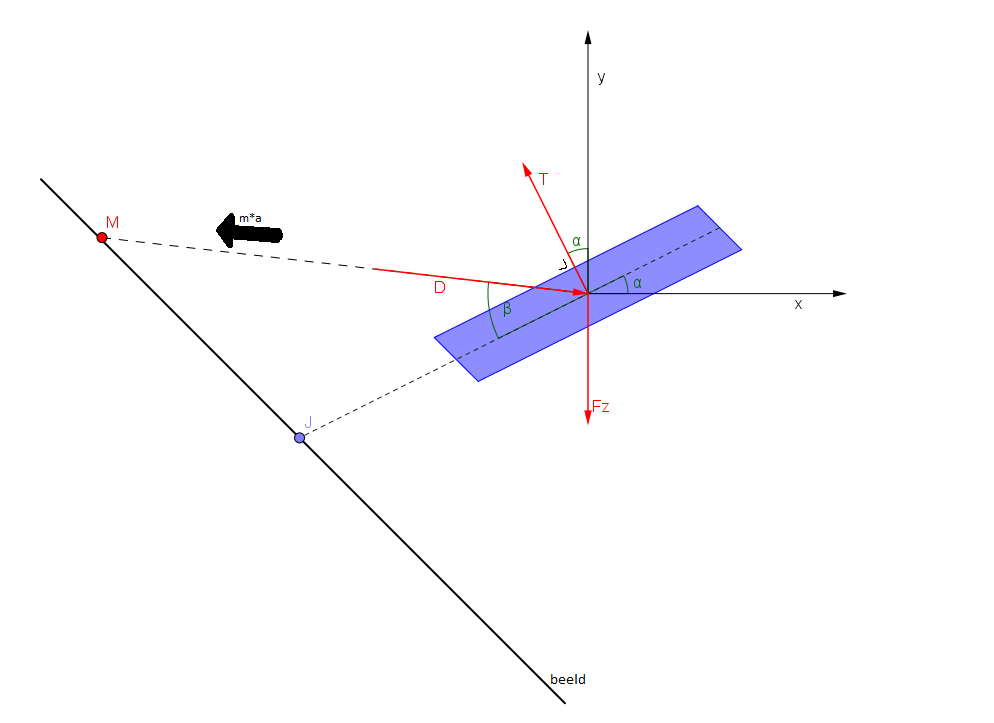
\includegraphics[width=0.5\textwidth]{GrafischeUitwerkingVanHoeveelheidThrustOnderBepaaldePitch.png}
	\caption{Grafische uitwerking van hoeveelheid thrust onder bepaalde pitch.}
	\label{fig:GrafischeUitwerkingVanHoeveelheidThrustOnderBepaaldePitch}
\end{figure}

\begin{equation}
\begin{cases}
T\cdot\sin(\alpha)-D\cdot\cos(\beta-\alpha) = m\cdot a\cdot\cos(\beta-\alpha)\\
T\cdot\cos(\alpha) - F_z - D\cdot\sin(\beta-\alpha) = m\cdot a\cdot\sin(\beta-\alpha)\\
\end{cases}
\end{equation}

\begin{equation}
\frac{T\cdot\sin(\alpha)-D\cdot\cos(\beta-\alpha)}{\cos(\beta-\alpha)} = \frac{T\cdot\cos(\alpha) - F_z - D\cdot\sin(\beta-\alpha)}{\sin(\beta-\alpha)}
\end{equation}

\begin{equation} \label{eq: thrustPitch}
T\cdot\sin(\alpha)\sin(\beta-\alpha) = T\cdot\cos(\alpha)\cos(\beta-\alpha)- F_z\cdot\cos(\beta-\alpha)
\end{equation}
Algemeen geldt er:
\begin{equation} \label{eq: gonio}
\cos(x+y) = \cos(x)\cos(y)-\sin(x)\sin(y)
\end{equation}
Door \ref{eq: gonio} toe te passen op vergelijking \ref{eq: thrustPitch} wordt volgende relatie afgeleid:
\begin{equation}
T = \frac{ F_z\cdot\cos(\beta-\alpha)}{\cos(\beta)}
\end{equation}

